\chapter{Microsoft Bot Framework}

The BotBuilder SDK is an open-source solution developed by Microsoft to write a chatbot in once and make it possible to connect that same chatbot to multiple channels. Examples are Skype, Slack, Facebook Messenger, etc.

\section{Business Model}

The Microsoft Bot Framework can be used in several ways. The base platform can be self-hosted on a server of choice. But to access the extra services, like spell checking, or recognizing user intents using Microsoft's LUIS (Language Understanding), an Azure subscription plan is required.

Azure is Microsoft's Cloud service that can be tailored to the customer's need. The customer can decide what modules or extra features he wants to add and calculate the price.

\begin{figure}[ht]
	\centering
	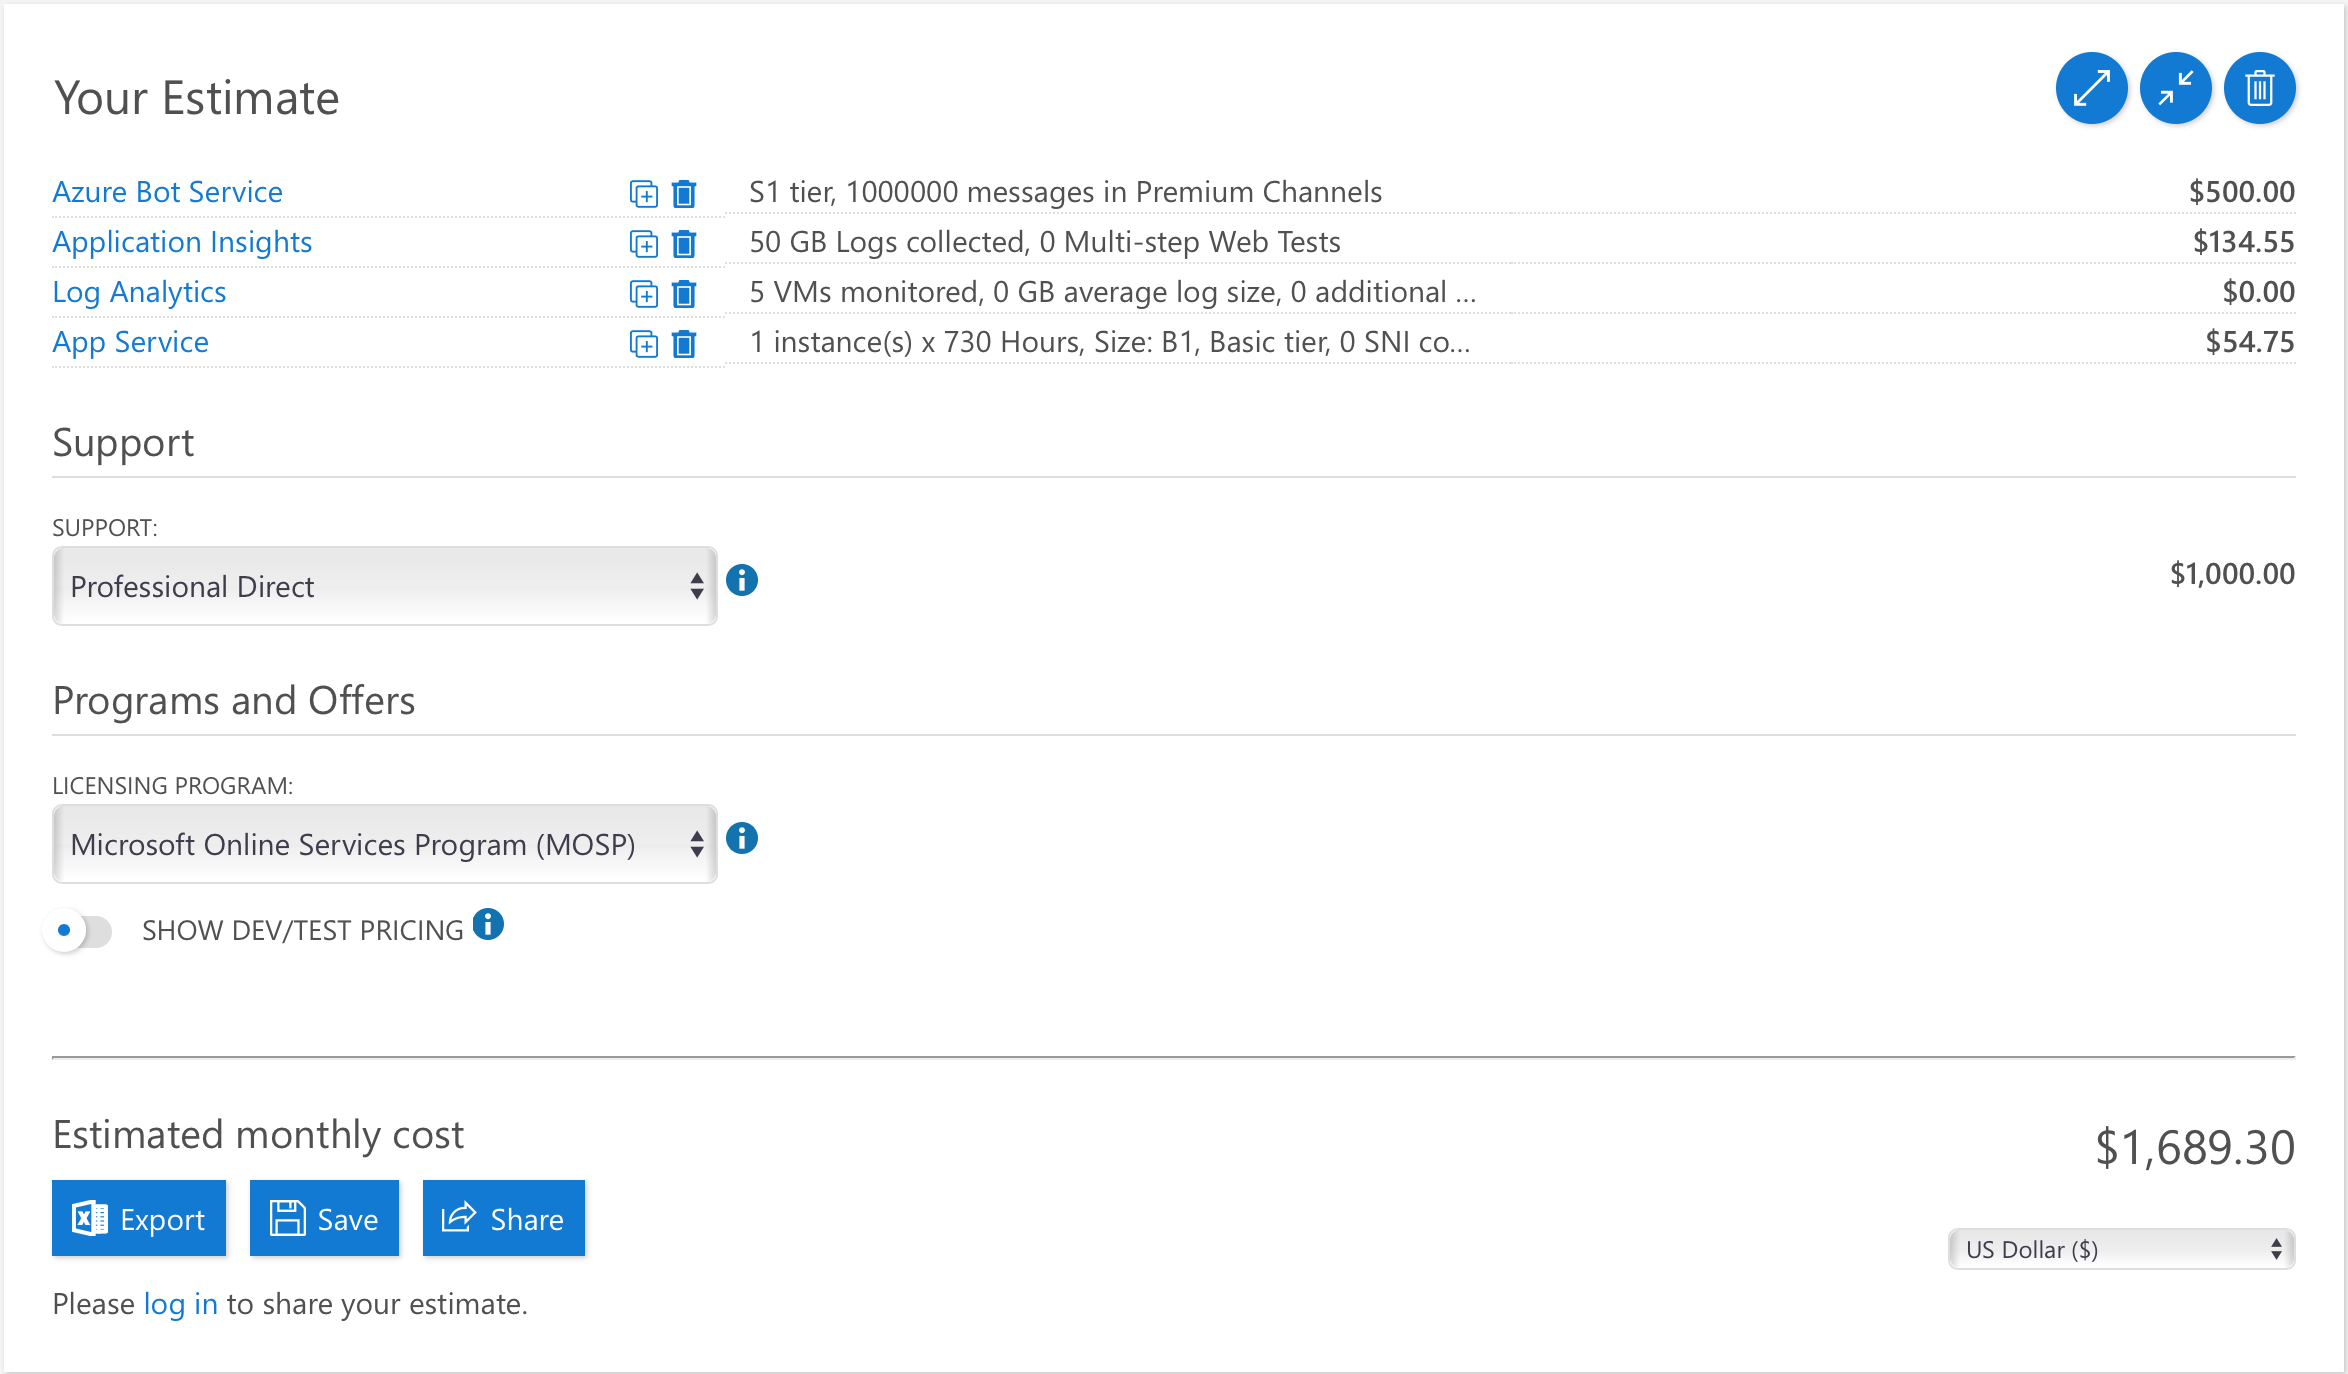
\includegraphics[width=\textwidth]{microsoft-azure-calculator-screen}\label{fig:microsoft-azure-calculator-screen}
	\caption{Microsoft's Azure Pricing Calculator~\cite{azure-pricing-calculator}}
\end{figure}

\section{Technical implementation}

Microsoft provides the bot framework for 2 languages: Node.JS and C\#. If C\# is used however, development can only be done inside of a Windows environment, or the limited online code editor.

One solution would be to use Node.JS in a code editor of choice. Preferably Visual Studio Code, Microsoft's cross-platform code editor. This way everything can be tailored and configured to the developer's needs.

\subsection{Developer environment}

Setting up a developer environment can be configured from scratch to be as complicated and complex as needed by the company or developer. Node.JS is an open-source, cross-platform JavaScript environment that can be run on a server. And in the end that's what a chatbot is, a sever API that responds to requests (messages or events from the user).

It's important to note that JavaScript or also called ECMAScript is a language that is advancing very quickly and Node.JS cannot keep up with all the newest yearly features. And all of the documentation involving the Bot Framework is written in ES5. However it's still possible to use all of the newest features of ECMAScript if you compile your code down the ES5.

The documentation on setting up an environment like this is very limited. Microsoft does not provide any instructions or boilerplates on how to set up an efficient environment. This makes for more freedom but increases the learning curve for a developer who wants to start coding a bot using newer ECMAScript features or the option to hot reload his code.

\subsection{Testing}

The bot can be tested locally or remotely on any platform using Microsoft's own Bot Emulator~\cite{microsoft-bot-emulator}, which is also open-source. This provides the developer with a live testing interface and information about everything the bot receives, including requests and the data that comes with them.

Speech Recognition is also supported for speech enabled bots. Sending system activities is another useful feature because it allows the developer to emulate user events like for example a user joining the conversation. Lastly, payment processing is supported as well to emulate a transaction.

\begin{figure}[ht]
	\centering
	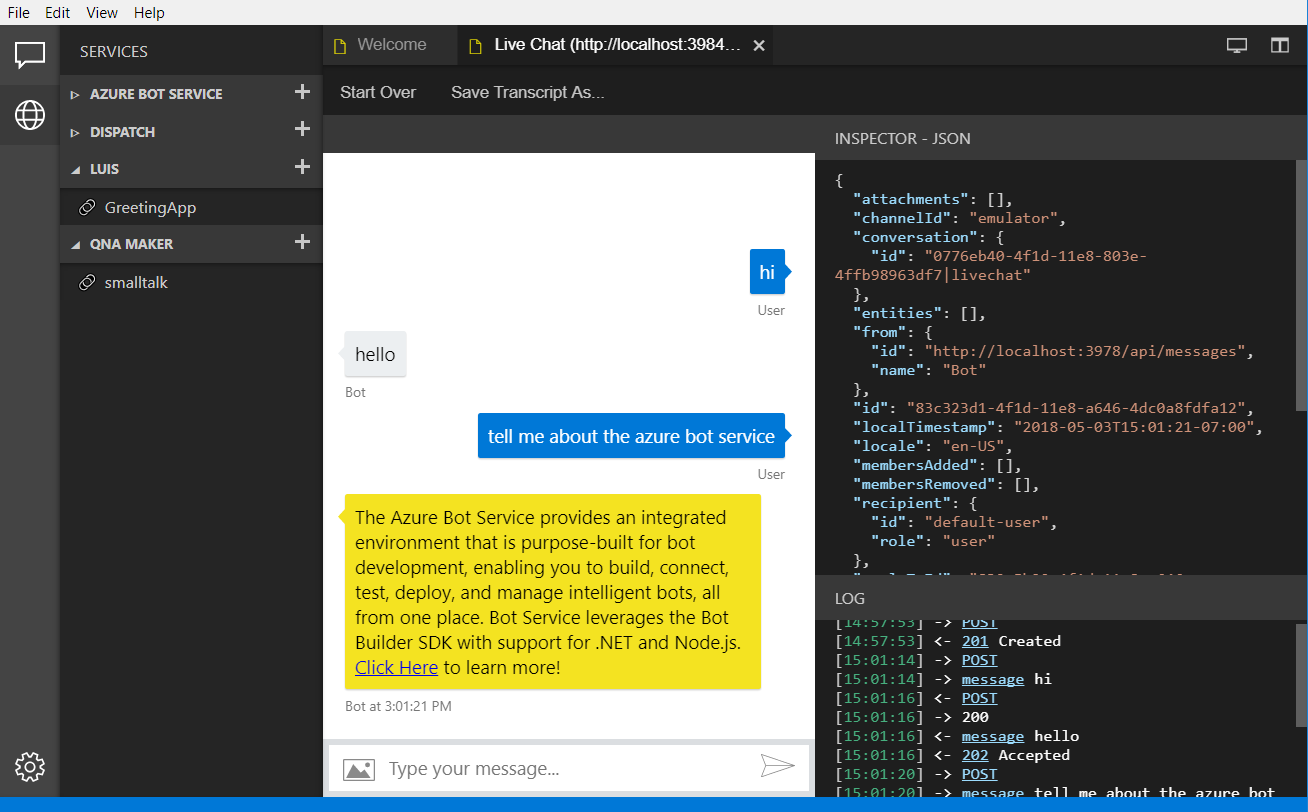
\includegraphics[width=\textwidth]{microsoft-bot-emulator}\label{fig:microsoft-azure-calculator-screen}
	\caption{Microsoft's Bot Emulator~\cite{microsoft-bot-emulator}}
\end{figure}